% Content for the test report for LSP-00-15

\subsection{Portal Aspect tests}

This test case exercises the LSP via the Portal Aspect only,
though it depends on the API Aspect for its operation.

It verifies the ability to perform a variety of basic catalog search types via the Portal.

Data for the test are primarily taken from the Object-like AllWISE (coadded) Source Catalog,
except as noted below.

\subsubsection{Step 1}

The tests were performed primarily from an Apple iMac computer running OS X 10.11.6,
connected to the Internet using a wired connection to the IPAC institutional network.
The Portal was accessed using the Firefox browser, in various versions.
Screenshots were taken from Firefox 59.

\subsubsection{Step 2}

A connection was established to the PDAC network environment using the NCSA VPN at \texttt{vpn.ncsa.illinois.edu}.

\subsubsection{Step 3}

\textbf{Step 3a:} The Portal was accessed at:

\begin{center}
\texttt{https://lsst-sui-proxy01.ncsa.illinois.edu/suit/}
\end{center}

\textbf{Step 3b:} The test case instructs that cone searches of 300 arcsecond radius be performed.
The Portal UI deployed on the PDAC (unnecessarily) limited cone searches to a 100 arcsecond radius,
so that is what was used.
See LSP-00-20 for additional discussion.

Cone searches of a 100 arcsecond radius around (\emph{ra}, \emph{dec}) = (0,0) were performed on the three tables mandated, with the NEOWISE Year 1 Single-Epoch Photometry table used as the Source-like table.
All columns were requested (i.e., \texttt{SELECT *}).
For the Object-like and Source-like tables the string \verb|source_id| column was used for choosing the ID mandated in the test specification.
For the Forced-Source-like table this column was not available and the numeric \verb|cntr| column was used instead.

All searches took approximately 1-2 seconds to execute and display results.

\begin{table}[h]
\centering
\begin{tabular}{l r l l}
PDAC WISE table & Rows & Selected ID & File \\ \hline
Object-like \verb|allwise_p3as_psd| & 37 & \verb|0000p000_ac51-032654| & \verb|step3b-Object.tbl| \\
ForcedSource-like \verb|allwise_p3as_mep| & 1,313 & \verb|100010333930023| & \verb|step3b-ForcedSource.tbl| \\
Source-like \verb|neowiser_yr1_p1bs_psd| & 394 & \verb|44373a126-005201| & \verb|step3b-Source.tbl| \\
\end{tabular}
\caption{Cone search results from selected PDAC WISE tables}
\label{tab:lsp-00-15-cone-results}
\end{table}

The table-download feature of the UI was used to download the files noted in the table,
preserved in the repository \verb|DMTR-52/lsp-00-15|.

\begin{figure}
  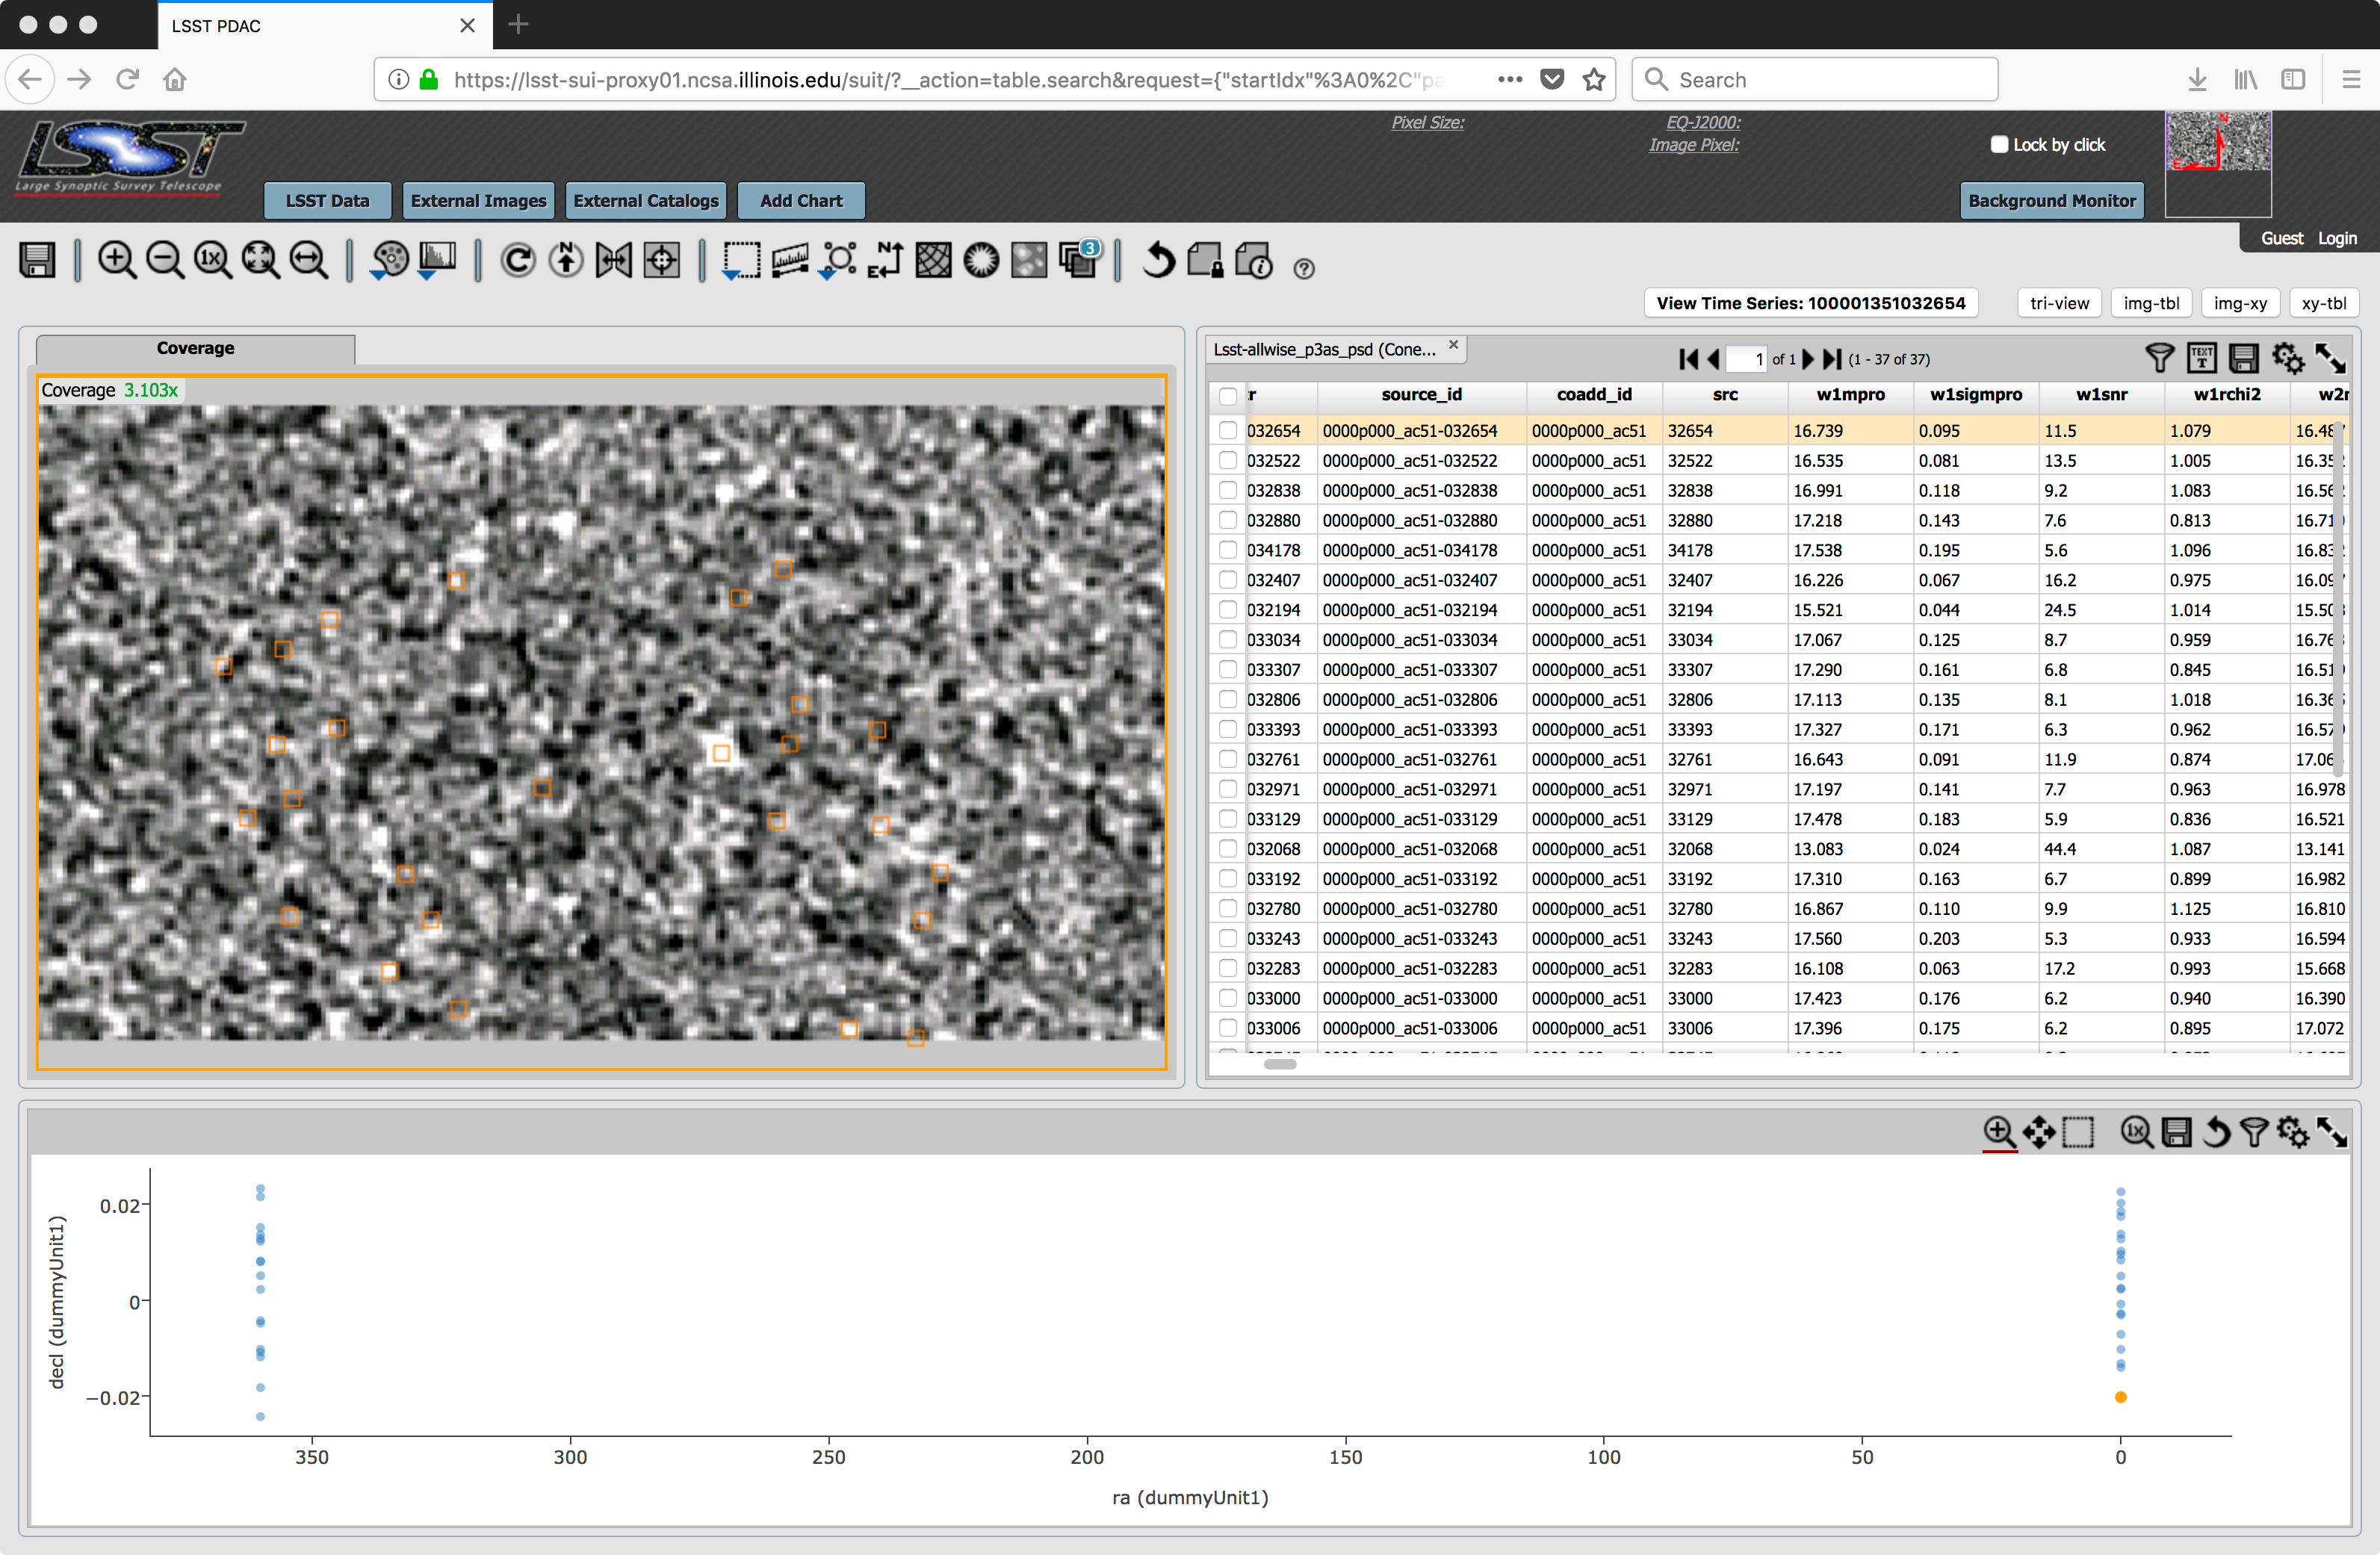
\includegraphics[width=\linewidth]{lsp-00-15/step3b-Object.png}
  \caption{Query results for the Object-like AllWISE Source Catalog}
  \label{fig:lsp-00-15-cone-Object}
\end{figure}

\begin{figure}
  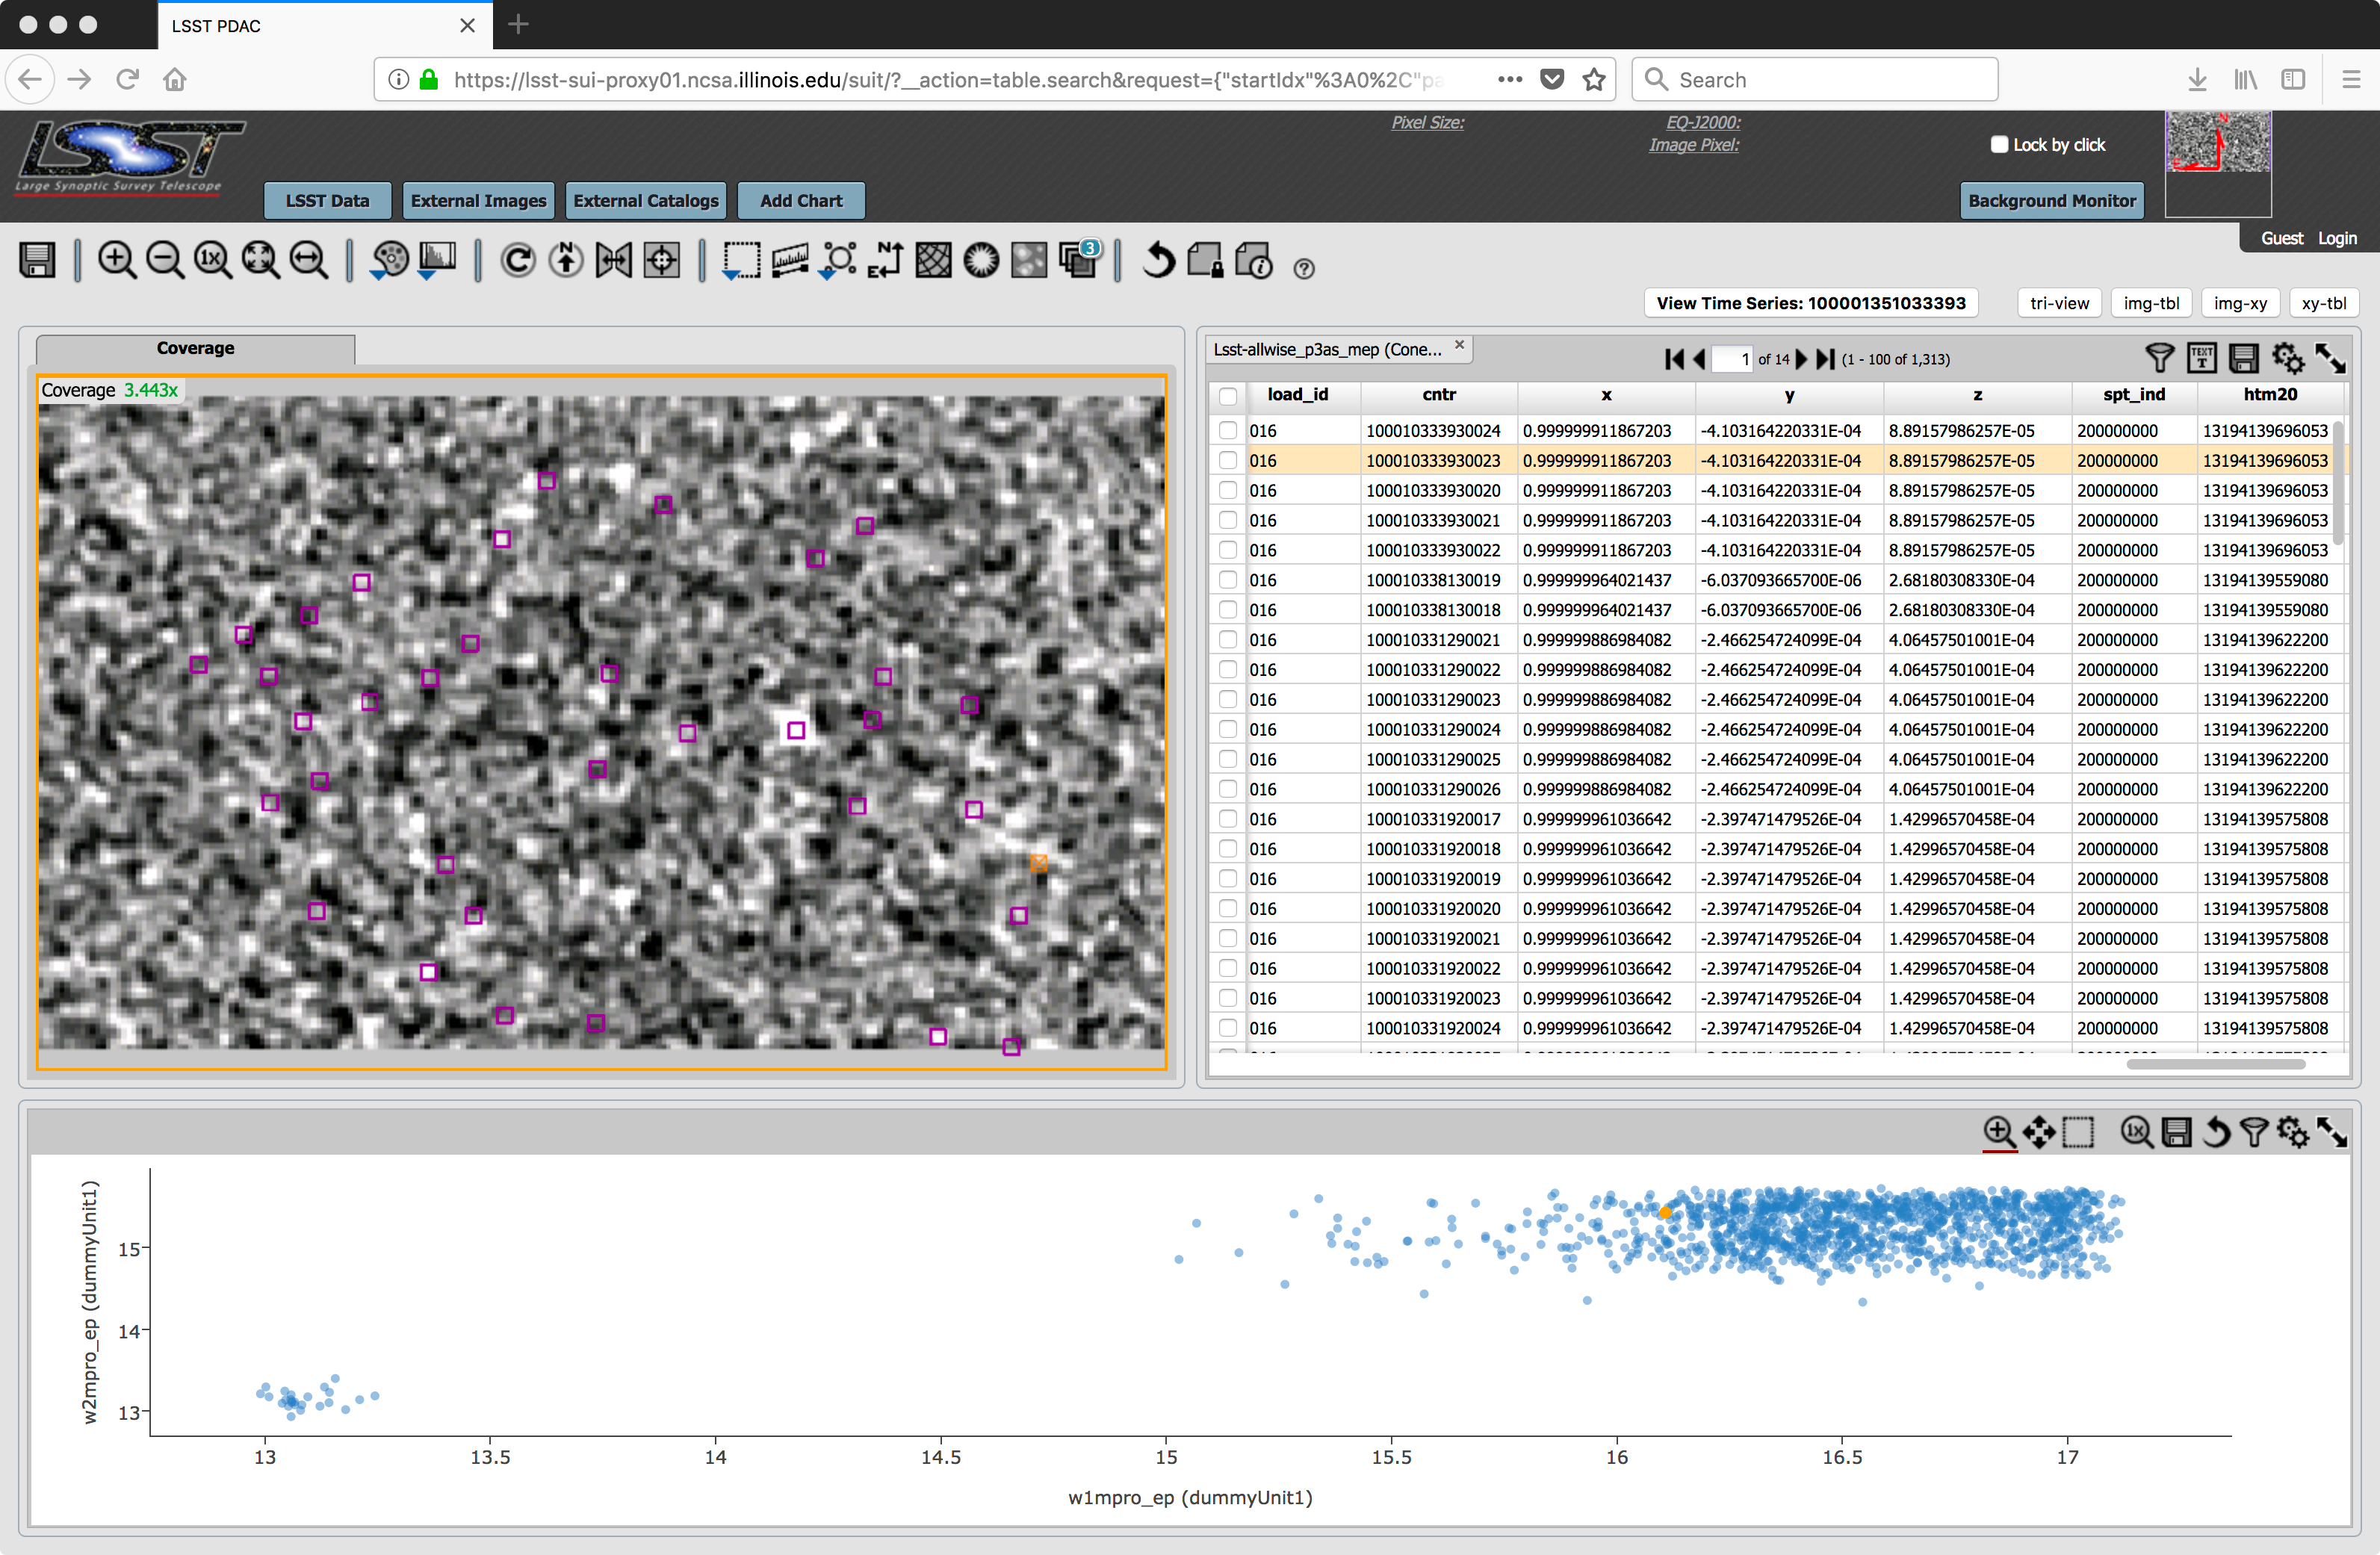
\includegraphics[width=\linewidth]{lsp-00-15/step3b-ForcedSource.png}
  \caption{Query results for the ForcedSource-like AllWISE Multi-Epoch Photometry table}
  \label{fig:lsp-00-15-cone-ForcedSource}
\end{figure}

\begin{figure}
  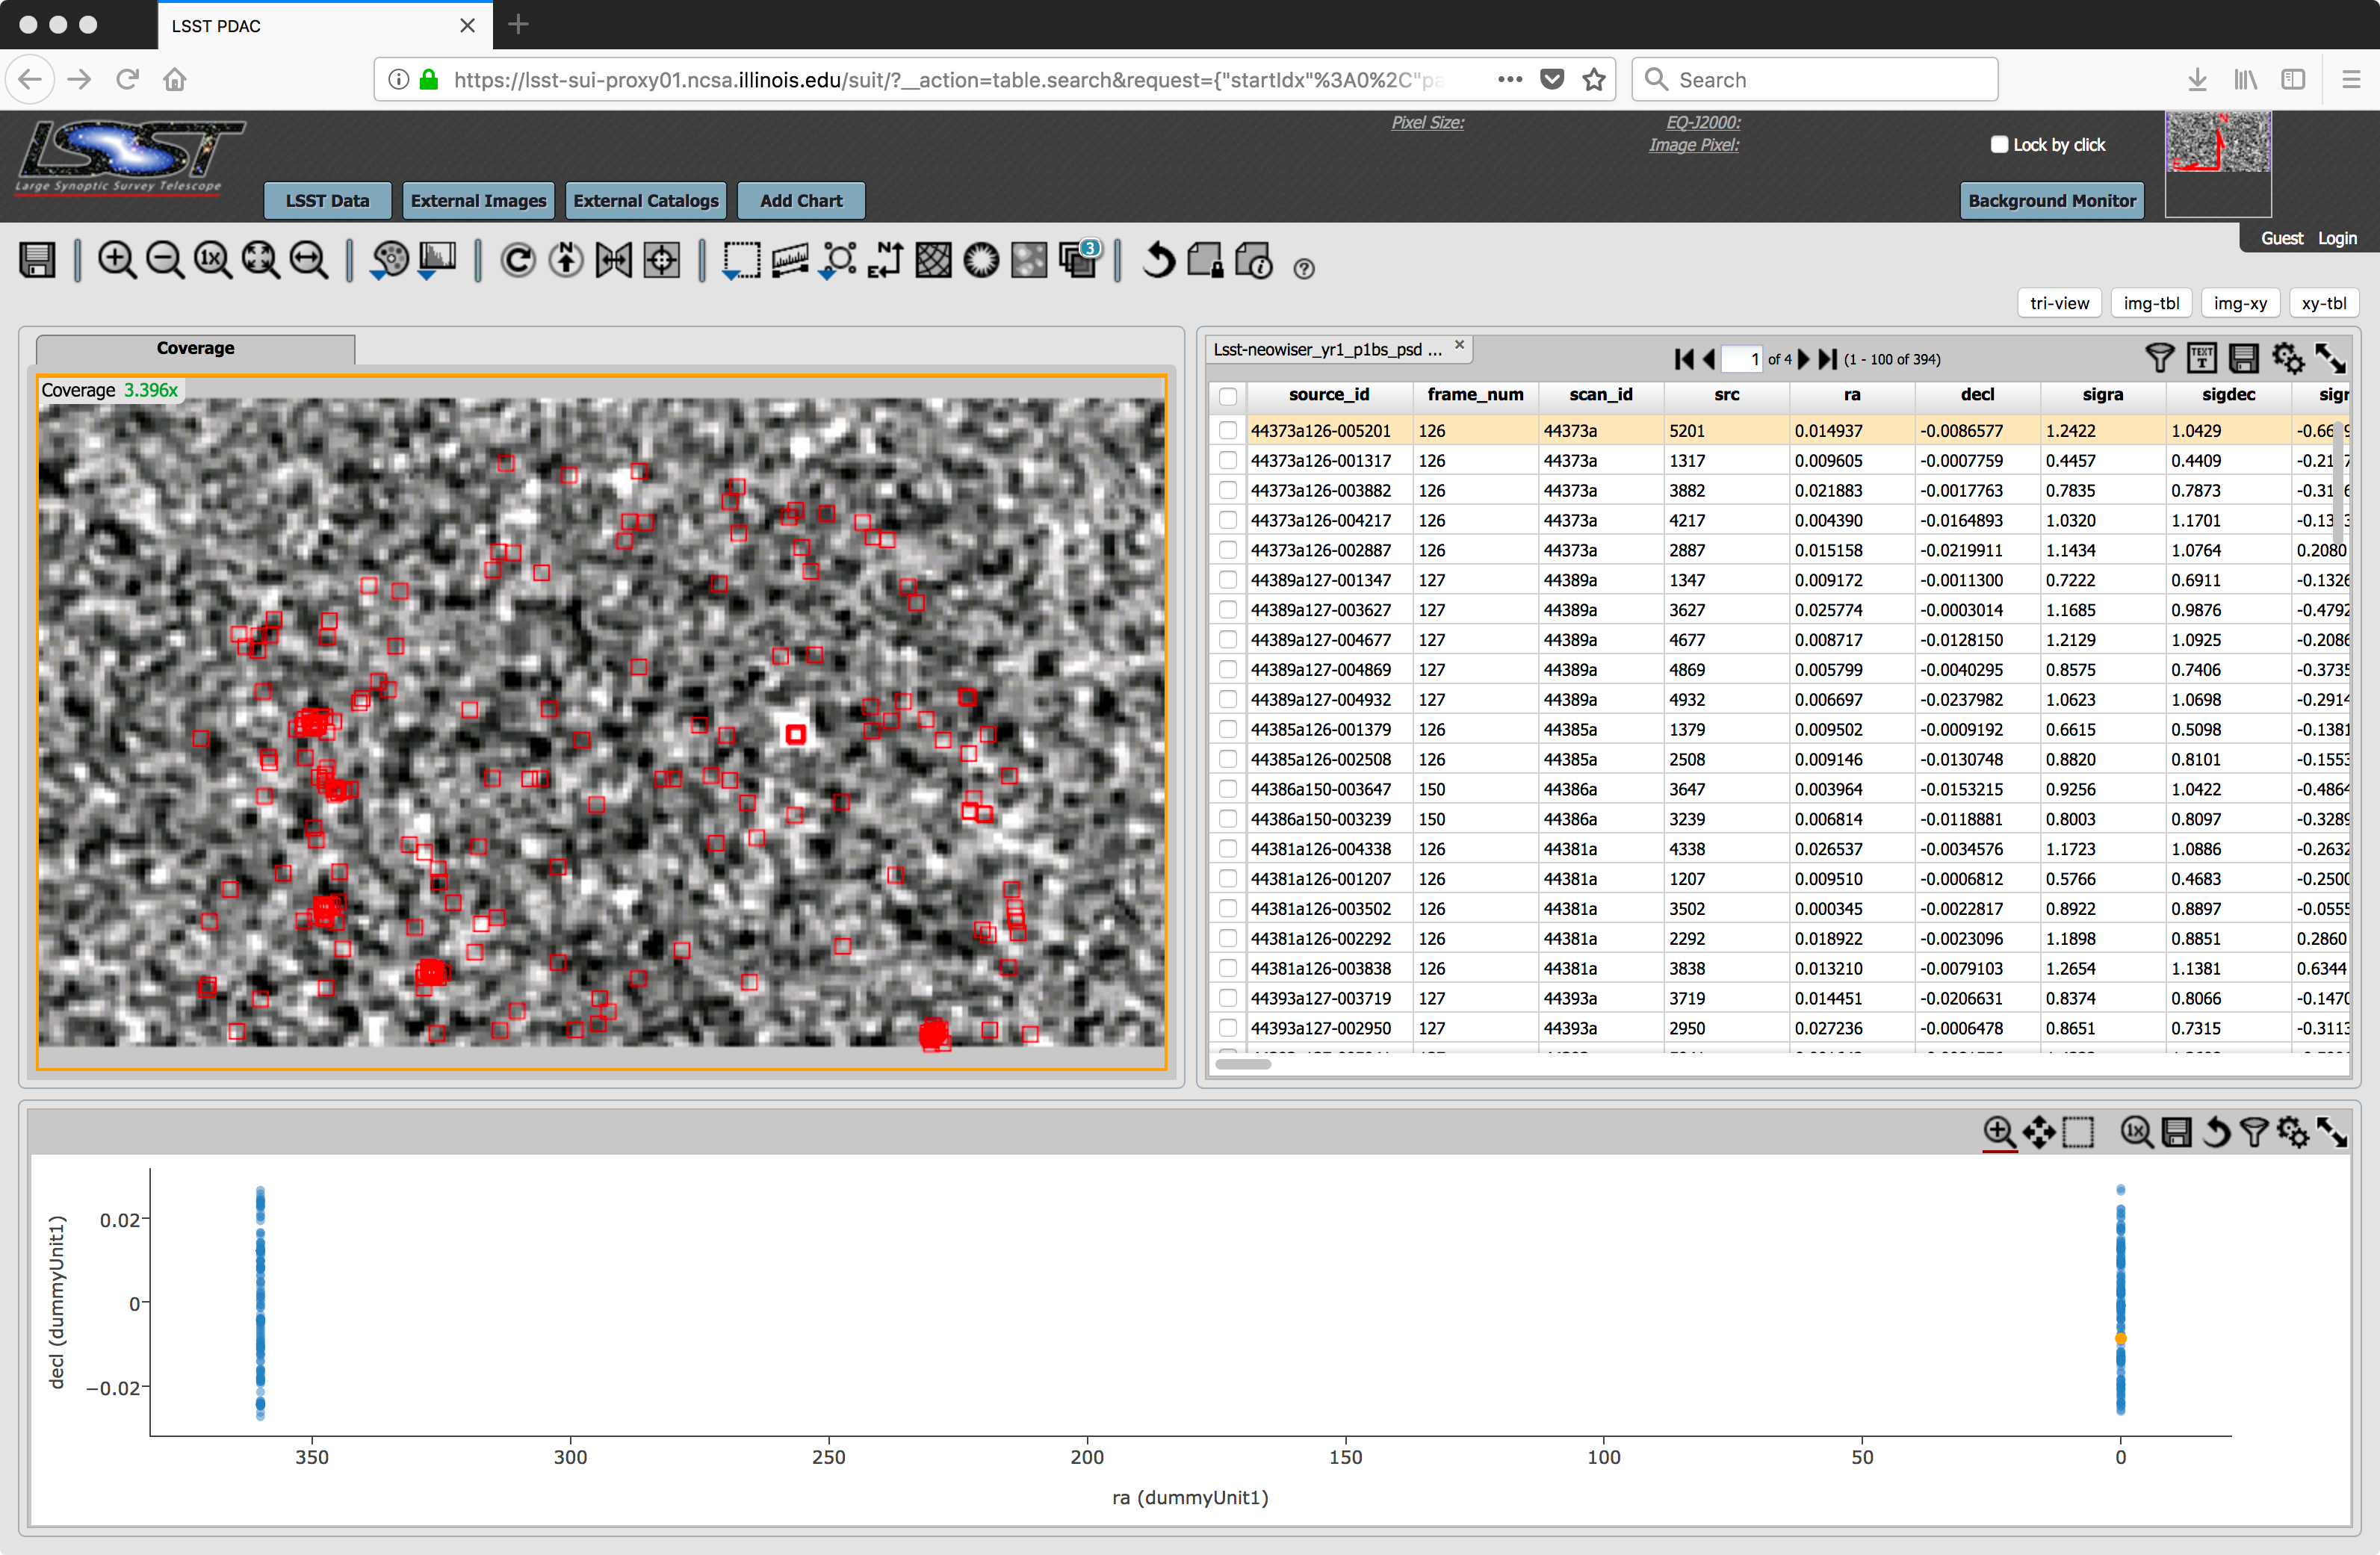
\includegraphics[width=\linewidth]{lsp-00-15/step3b-Source.png}
  \caption{Query results for the Source-like NEOWISE Year 1 Single-Epoch Source Catalog}
  \label{fig:lsp-00-15-cone-Source}
\end{figure}



\textbf{Step 3c:} The multi-object search functionality of the UI was tested using a nominal 30 arcsecond search radius for each target in \verb|LDM-540/test-scripts/lsp-00-15-coords.tbl|,
which was uploaded to the UI.
(The target list file had been generated using standard techniques for generating a uniform distribution of 100 random points on a sphere.)
Note that the file name was changed from the originally suggested one in LDM-540 to help make clear that this file is in IPAC Table form,
the only form currently accepted by the UI.
The IPAC Table restriction should be reconsidered as part of the further development of the system.
VOTable, at least, should be supported, and ideally also a more free-form input.

The test succeeded, finding multiple source for most targets, but requiring 14 seconds to perform a 100-object search.
The test confirmed the ability to carry forward additional columns from the target table, beyond the \verb|ra| and \verb|dec|,
to the result table, and associate them correctly with multiple search hits.
A feature present in the equivalent IRSA capability was missing, however: the preservation of a row index from the original target table.
This is a nice feature of the IRSA Viewer application's implementation.
The result table was preserved as \verb|DMTR-52/lsp-00-15/step3c-Objects.tbl|.

The normal implementation of multi-object searches is as a user table upload followed by a spatial join in a database.
The current implementation of this feature in the Portal Aspect, however,
required a workaround for the inability to upload user tables to the DAX system at this time.
It therefore operates by iterating over searches one target at a time, inside the Portal Aspect server,
and therefore performing many separate calls to the API Aspect.
This feature will get reimplemented once the database systems provide the requisite underlying support.
With the parallelism of Qserv, it can be expected to execute much more efficiently for substantially
larger numbers of targets.

\begin{figure}
  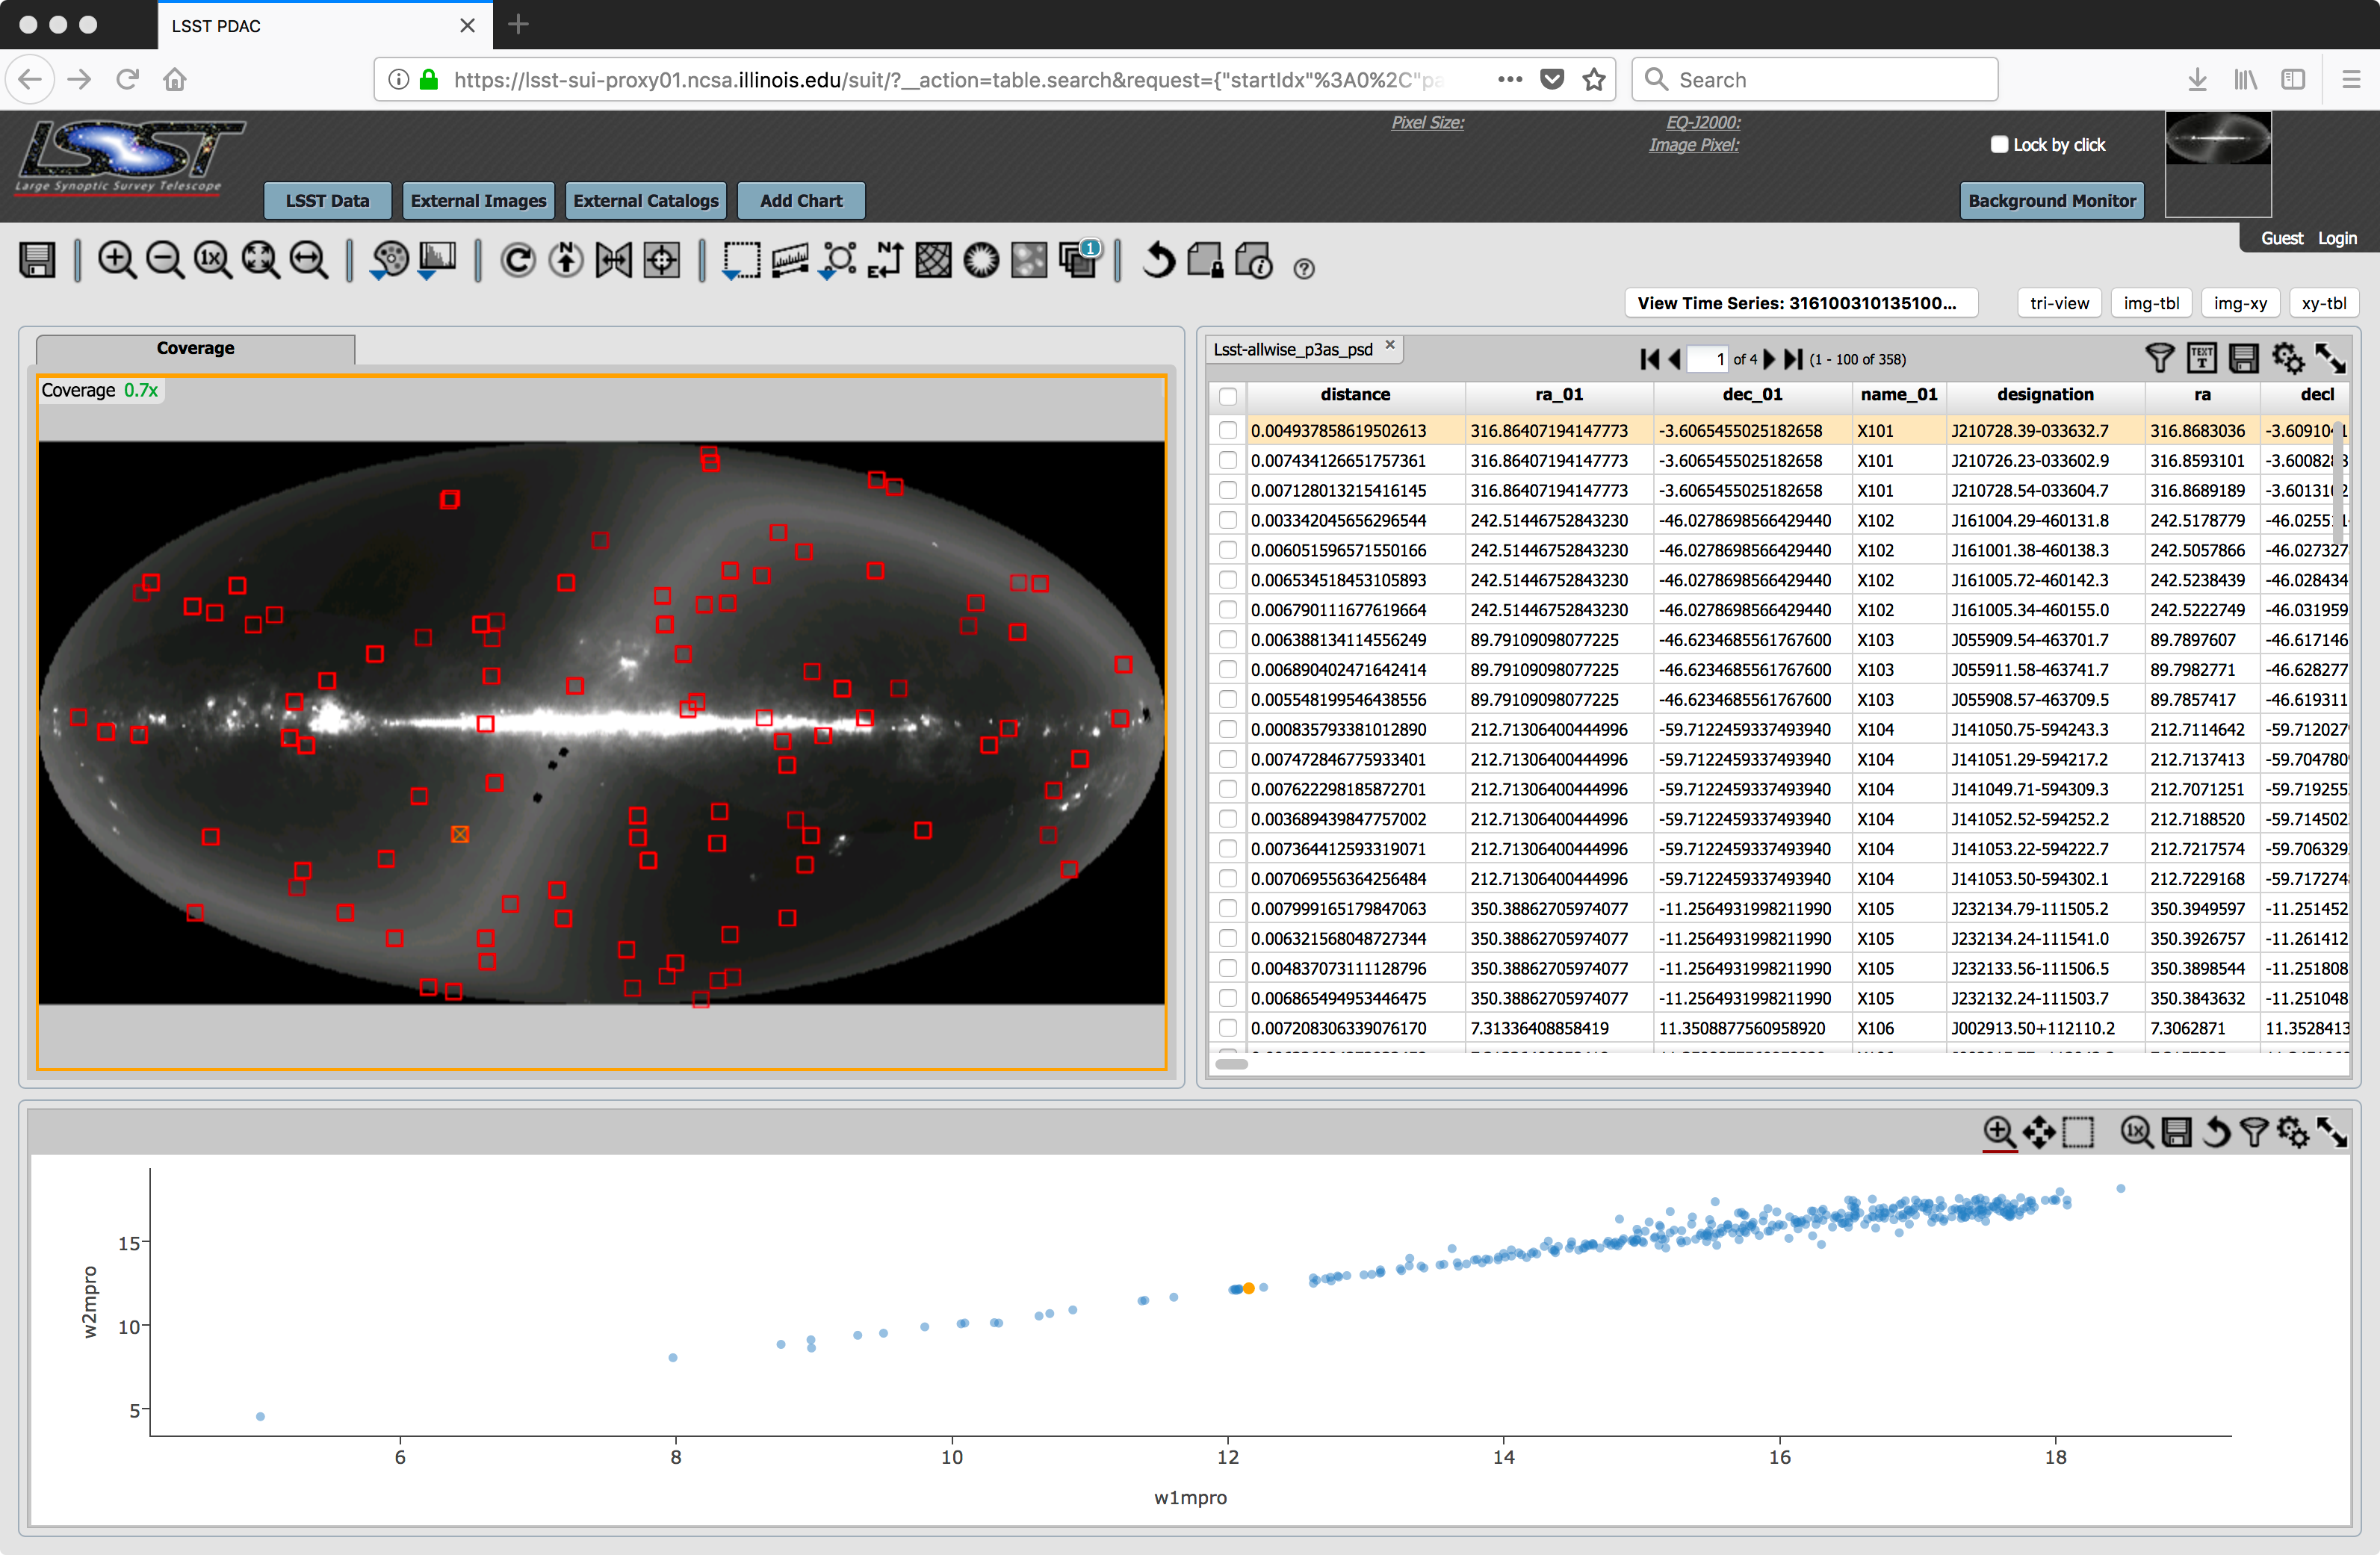
\includegraphics[width=\linewidth]{lsp-00-15/step3c-Objects.png}
  \caption{Query results for the 100-target search on the Object-like AllWISE Source Catalog}
  \label{fig:lsp-00-15-multi-search}
\end{figure}


\textbf{Step 3d:} The ``All Sky'' search form was used to perform the identifier-based searches required.
For the Object-Like and Source-like searches the search was performed on the \verb|source_id| field,
was successful and completed essentially instantaneously, consistent with the timings seen in LSP-00-05.

This did require typing the ``constraint'' in the search form in this format: ``\verb|='0000p000_ac51-032654'|'',
which is not natural.
Typing just the string itself was not successful, even though this is an intuitive thing to attempt,
and the resulting error message requires SQL knowledge to interpret.
This should be improved.

\begin{figure}
  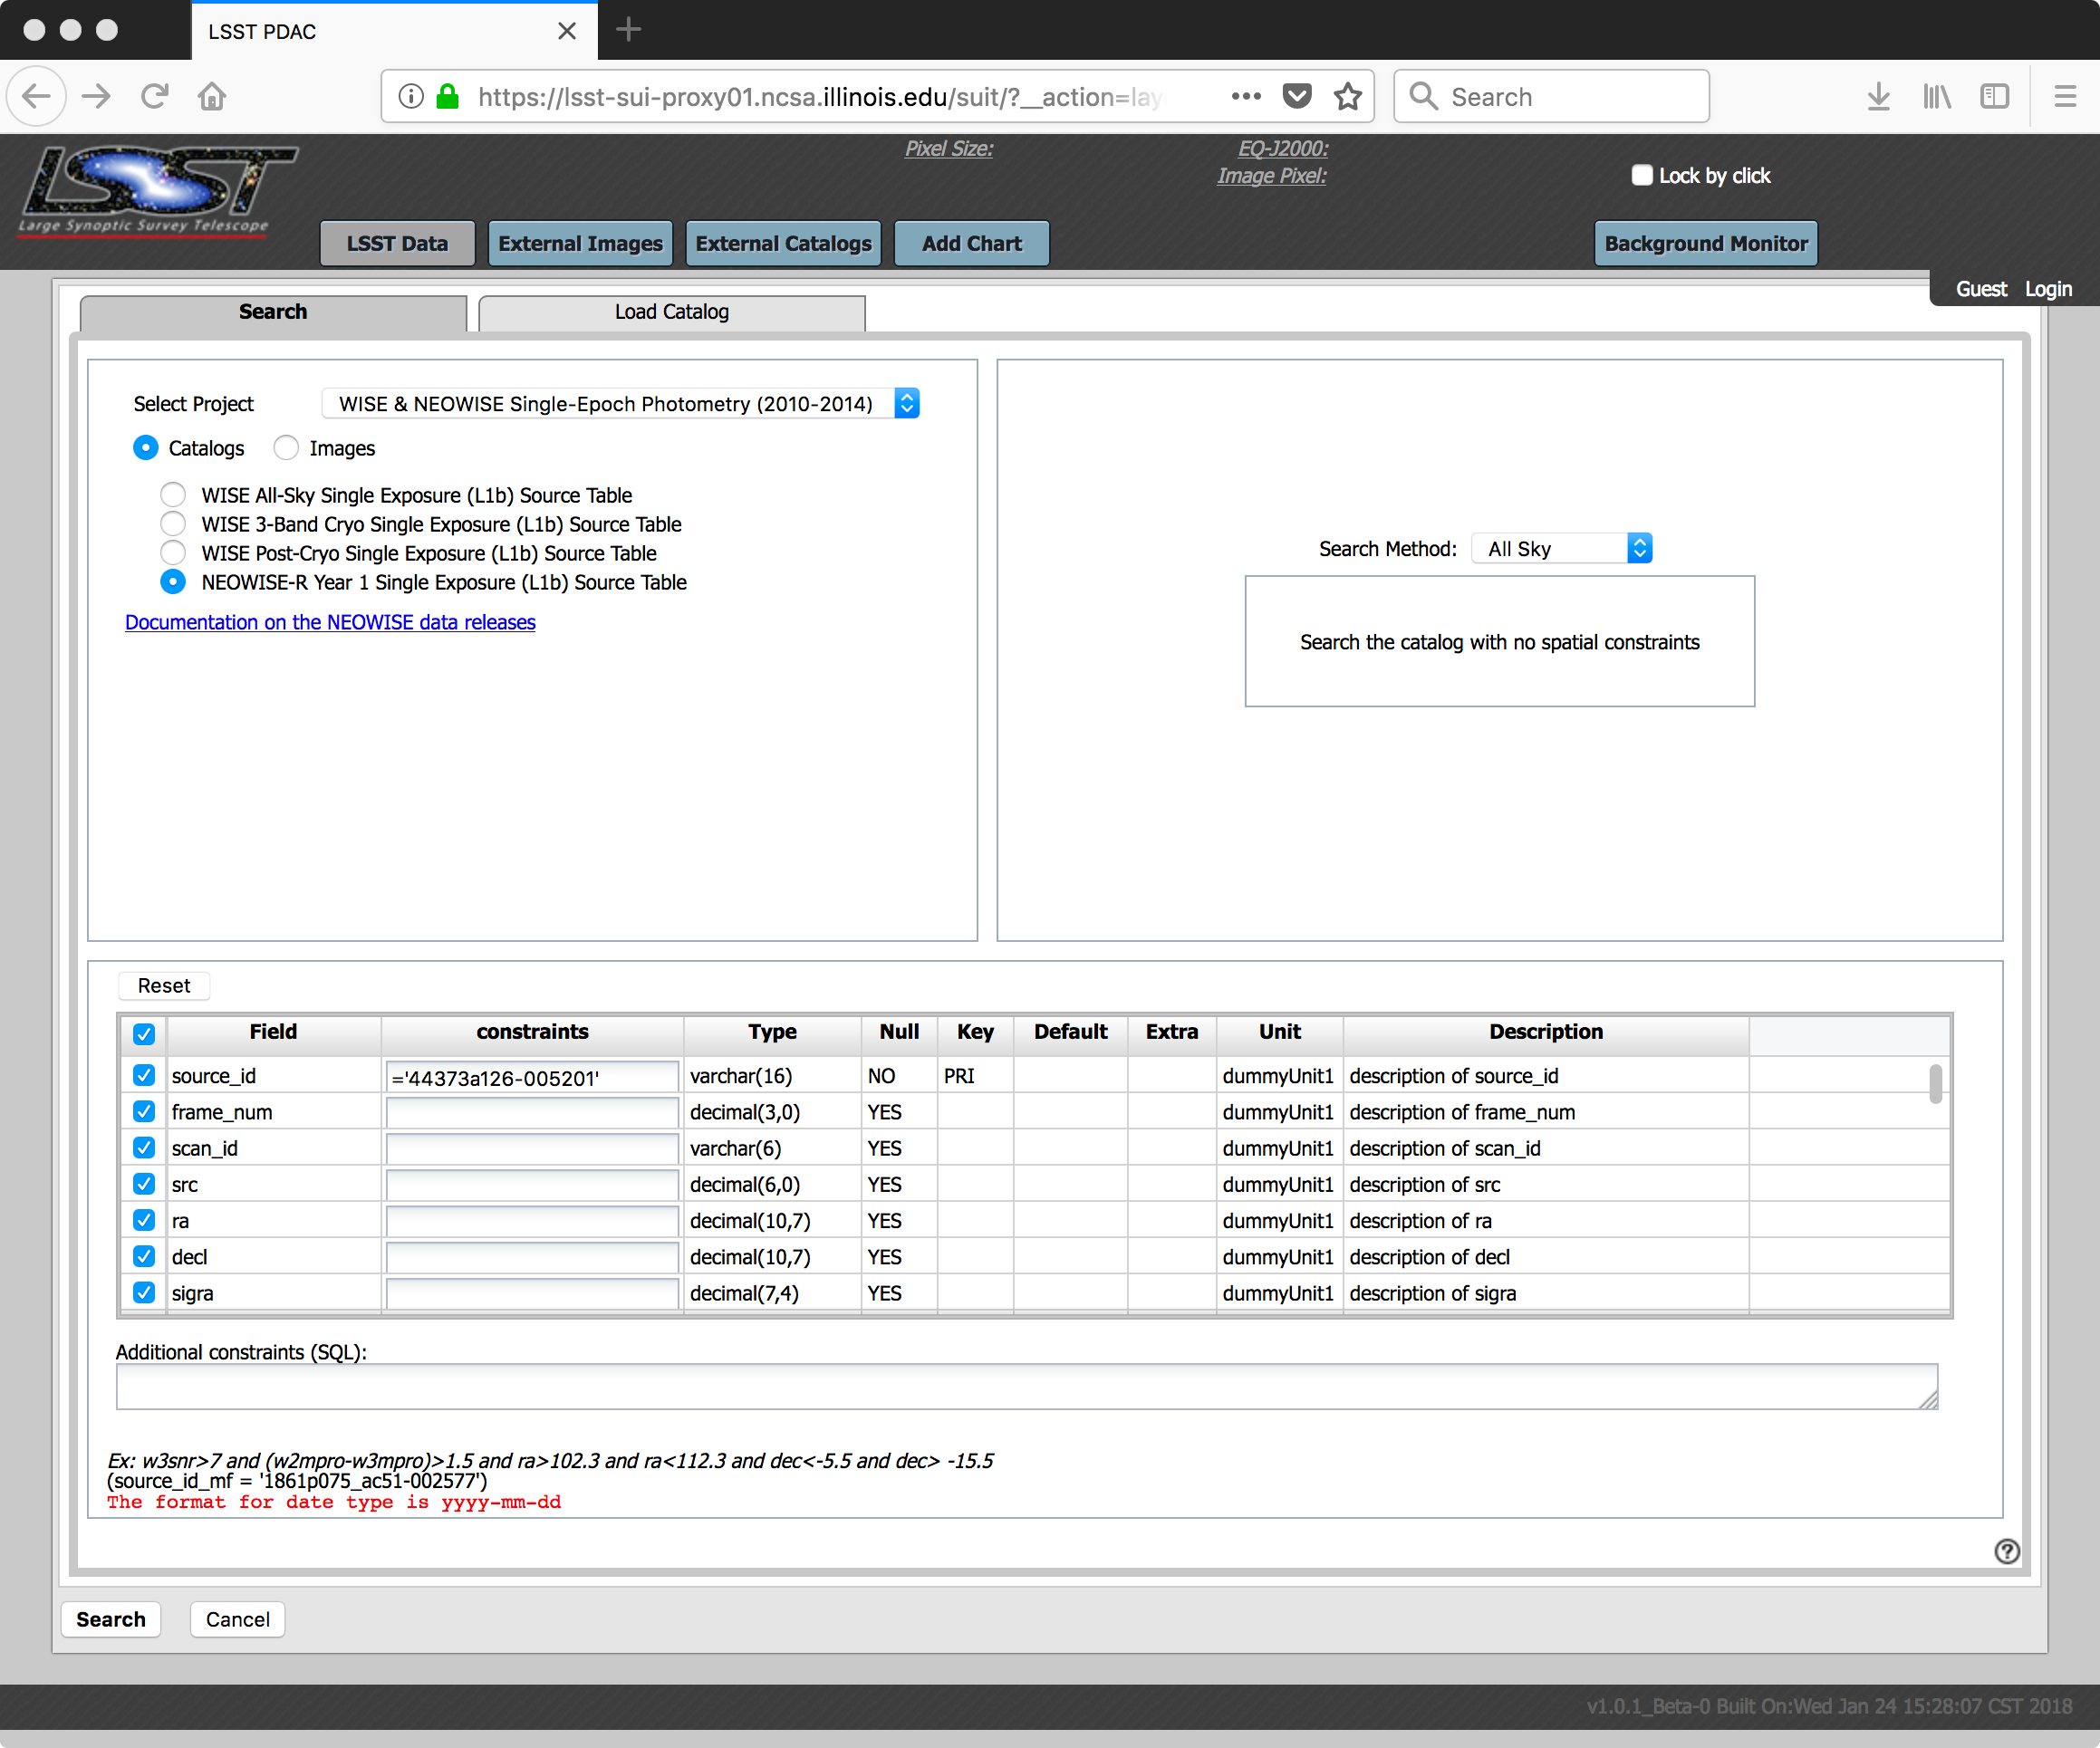
\includegraphics[width=\linewidth]{lsp-00-15/step3d-Source-search.png}
  \caption{Search screen for a search-by-ID on the Source-like catalog}
  \label{fig:lsp-00-15-source-id-search}
\end{figure}

Search results were preserved as files \verb|DMTR-52/lsp-00-15/step3d-Object.tbl| and \verb|DMTR-52/lsp-00-15/step3d-Source.tbl|.

For the ForcedSource-like table an attempt to search on the value of \verb|cntr| appeared to trigger a table scan and was not feasible as an interactive query.
Further investigation revealed that this table is not indexed on \verb|cntr| or any other per-row unique key at this time.

It was, however, possible to manually search on the ForcedSource-like table with the ID from the Object table, \verb|0000p000_ac51-032654|,
and obtain a 27-row light curve table.
(Note that a predefined workflow for this is also available in the UI and is exercised in LSP-00-35 below.)

Search results were preserved as files \verb|DMTR-52/lsp-00-15/step3d-lightCurve.tbl|.

\begin{figure}
  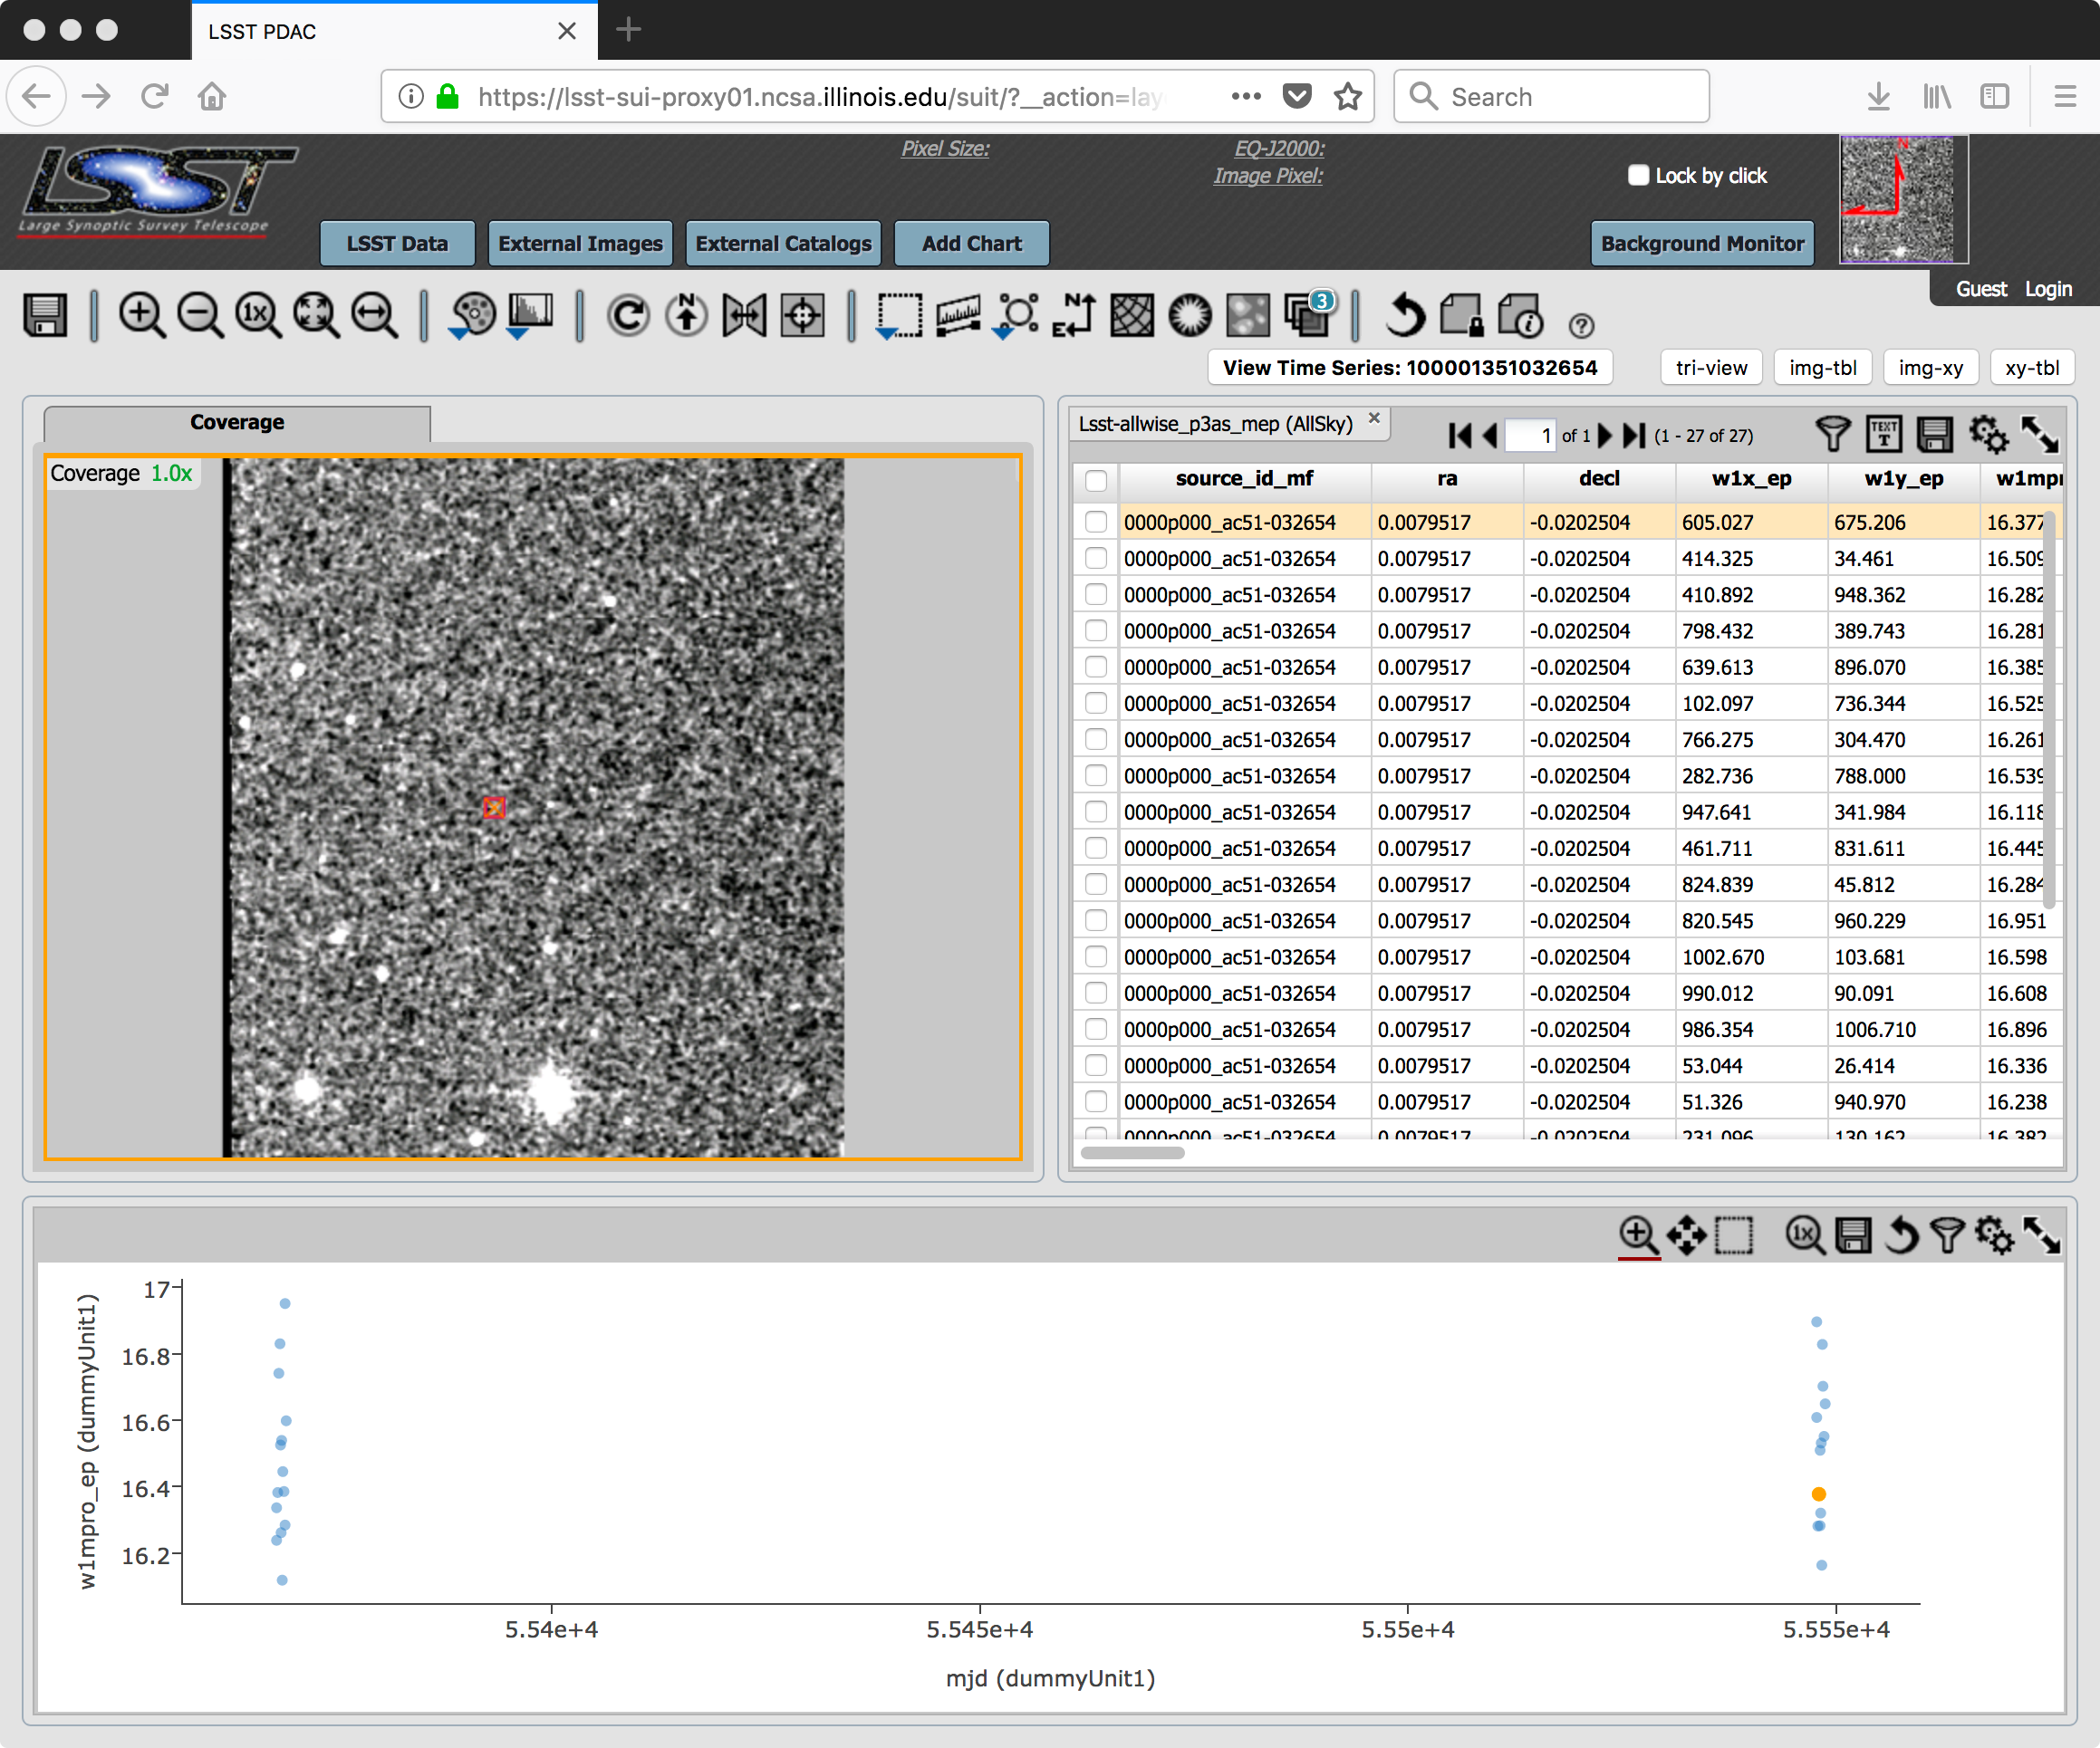
\includegraphics[width=\linewidth]{lsp-00-15/step3d-lightCurve-results.png}
  \caption{Results of a search-by-Object-ID on the ForcedSource-like catalog}
  \label{fig:lsp-00-15-lightCurve-results}
\end{figure}

